\documentclass[a4paper]{report}
\usepackage{geometry}
\usepackage{makeidx}
\usepackage{graphicx}
\usepackage{tabularx}
\usepackage[printwatermark]{xwatermark}
\usepackage{xcolor}
\usepackage{tikz}
\usepackage{multicol}
\usepackage{float}
\usepackage{listings}
\usepackage{color}
\usepackage{ifthen}
\usepackage{textcomp}
\usepackage{alltt}
\usepackage{ifpdf}
\ifpdf%
\usepackage[pdftex,
            colorlinks=true,
            linkcolor=blue,
            unicode
           ]{hyperref}
\else
\usepackage[ps2pdf,
            colorlinks=true,
            linkcolor=blue,
            unicode
           ]{hyperref}
\usepackage{pspicture}
\fi
\usepackage[utf8]{inputenc}
\usepackage{mathptmx}
\usepackage[scaled=.90]{helvet}
\usepackage{courier}
\usepackage{parskip}
\usepackage{sectsty}
\usepackage{booktabs}
\usepackage[titles]{tocloft}
\usepackage{fancyhdr}
\usepackage{scrextend}
\usepackage{afterpage}
\usepackage[nottoc,numbib]{tocbibind}

\renewcommand{\familydefault}{\sfdefault}

% A watermark for draft copies (remove as necessary)
%\newsavebox\mybox{}
%\savebox\mybox{\tikz[color=red,opacity=0.3]\node{DRAFT};}
%\newwatermark*[
%  allpages,
%  angle=45,
%  scale=6,
%  xpos=-20,
%  ypos=15
%]{\usebox\mybox}

% The geometry of all of our pages
\geometry{
 a4paper,
 total={170mm,237mm},
 left=20mm,
 top=30mm,
}

% Define the thickness of the header and footer rules
\renewcommand{\headrulewidth}{1pt}
\renewcommand{\footrulewidth}{1pt}

% A command to provide a completely blank page
\newcommand\blankpage{%
    \null%
    \thispagestyle{empty}%
    \addtocounter{page}{-1}%
    \newpage}

% A method defined in fancyhdr documentation for twosided blank pages before a chapter start
%\makeatletter
%\def\cleardoublepage{\clearpage\if@twoside \ifodd\c@page\else
%  \hbox{}
%  \vspace*{\fill}
%  \begin{center}
%  This page is intentionally left blank.
%  \end{center}
%  \vspace{\fill}
%  \thispagestyle{empty}
%  \newpage
%  \if@twocolumn\hbox{}\newpage\fi\fi\fi}
%\makeatother

% Define the header and footer for all pages except the title and blank pages
\fancypagestyle{plain}{
  \fancyhf{}
  \fancyhead[L]{SAFEcrypto}
  \fancyhead[R]{\leftmark}
  \fancyfoot[R]{\thepage}
}
\pagestyle{plain}

% Configure indexing of the TOC to a depth of 3 levels
\makeindex
\setcounter{tocdepth}{3}

\makeatletter% Set distance from top of page to first float
\setlength{\@fptop}{5pt}
\makeatother

\begin{document}
\hypersetup{pageanchor=false}

% THe title page
\begin{titlepage}
\vspace*{7cm}
\begin{center}

\includegraphics[scale=0.5]{../Resources/SAFEcrypto.png}\\
\vspace*{1cm}
{\huge Software Coding Guidelines}\\
\vspace*{1cm}
{\LARGE SAFEcrypto: Secure Architectures of Future Emerging Cryptography}\\
\vspace*{0.5cm}
{\small \today}\\
\end{center}
\end{titlepage}

% Intentionally leave a blank page after the title/cover page
\afterpage{\blankpage}
\clearpage

% Use Roman numbers for any pages prior to the Introduction
\pagenumbering{roman}

% Insert a Revision History table (MUST BE MANUALLY EDITED)
\begin{table}[t!]
\centering
\caption{Revision History}
\label{my-label}
\begin{tabularx}{\textwidth}{lllX}
\toprule
\textbf{Date} &\textbf{Version} &\textbf{Author~(s)} &\textbf{History}  \\
\midrule
3rd August 2016 &1.0 &N.Smyth &Initial Draft  \\
\midrule
22nd March 2017 &1.1 &N.Smyth &Expanded using MSc Cyber Security lecture notes \\
\midrule
 &  &  & \\
 \bottomrule
\end{tabularx}
\end{table}

\clearpage

% Insert a Table of Contents
\tableofcontents

% From this point onwards insert a blank page WHERE NECESSARY to ensure chapters start on the right
%\clearpage{\pagestyle{empty}\cleardoublepage}

% Use Arabic numbering from this point onwards
\pagenumbering{arabic}
\hypersetup{pageanchor=true}


\chapter{Introduction}
\label{ch_introduction}

This Introduction provides an overview of the entire \textit{Software Coding Guidelines} document for SAFEcrypto.
It includes the purpose, scope, definitions, acronyms, abbreviations, references and a document overview.

\section{Purpose}
SAFEcrypto will provide a new generation of practical, robust, and physically secure post-quantum cryptographic functions. Work Package 6 will develop a suite of software routines to implement the lattice-based constructions identified in Work Package 4 of the SAFEcrypto project.

A well designed system can be rendered useless at the implementation stage if poor coding and weak coding practices are used. All coding environments, no matter how small the project is, must have a set of policies and guidelines that are well documented and enforced. The adoption of a uniform set of rules and guidelines will promote robust coding practices that achieve software assurance.

Coding Standards exist for a range of languages, the Software Engineering Institute (SEI) contains secure coding standards for C, \verb!C++!, Java, Perl and Android and is an excellent resource for information around software assurance. Typically network and systems level code is written in C/\verb!C++! and the reality is a large amount of cryptographic code and security protocols are written in these languages.

While these are some of the most powerful and performance enhancing languages available, they are also amongst the most dangerous. The danger lies in the flexibility of these languages, and that they are at a lower level of compilation. As the level of language compilation gets lower bugs and vulnerabilities become more difficult to detect.

The SEI Secure Coding Standards contain a comprehensive wiki of rules and recommendations:

\begin{enumerate}
	\item Rules provided are normative requirements for code violations have the potential to introduce a security vulnerability and are detectable through code analysers.
	\item Recommendations provide guidance on increasing software assurance at a code level these are not compulsory and are suggestions that can increase the level of assurance within code. Recommendations are typically enforced in accordance with the product requirements, for example high grade security products will normally enforce many of the recommendations. A system that has critical safety requirements may go even further by enforcing safety standards, e.g. a ban on dynamic memory etc.
\end{enumerate}

This document provides a set of secure coding guidelines and principles that will ensure that the software development process adheres to best practices in trustworthy software development. In addition to secure coding guidelines some rules with regards to style guidelines are also provided, this is to provide a consistent and readable source code package that will be released into the public domain. In addition the build system and various build tools are described that will be used to automate the process of rule checking.

\section{Scope}
The scope of this document includes the entire SAFEcrypto software development lifecycle including architecture and design, implementation, build infrastructure and testing strategy. A well-documented and enforceable coding standard is an essential element of coding in the C programming language.

A SAFEcrypto coding standard encourages developers to follow a set of rules that benefit the SAFEcrypto project in terms of producing software that is secure, reliable and robust. These rules can be checked manually (e.g.\ code reviews) or using automated processes incorporated into the build system (e.g. Lint, CppCheck).


\section{Definitions, Acronyms and Abbreviations}
\begin{labeling}{SAFEcrypto}
\item [SAD] Software Architecture Document
\item [SAFEcrypto] Safe Architectures of Future Emerging Cryptography
\item [WP\textit{N}] Work Package \textit{N}
\end{labeling}

\section{References}
The following documents should be read in conjunction with this \textit{Software Architecture Document}:

\begin{itemize}
\item SAFEcrypto: Secure Architectures of Future Emerging Cryptography, H2020-ICT-2014--1~\cite{safecrypto_overview}
\item SAFEcrypto: Software Requirements Specification, Version 1.0, April 22 2016~\cite{safecrypto_srs}
\item SAFEcrypto: Software Architecture Document, Version 1.0,~???
\end{itemize}

\section{Overview}
This document consists of 5 sections which are described below:

\begin{itemize}
\item Section 1 is simply an introduction to the coding guidelines of the SAFEcrypto software system.
\item Section 2 identifies the goals and constraints of the coding guidelines.
\item Section 3 describes an overview of the proposed software system.
\item Section 4 provides a set of rules for C programming language development.
%\item Section 5 discusses the automated tools that will be incorporated into the build system.
%\item Section 6 provides a description of the code review process.
\item Section 5 is a bibliography of the references used to create this document.
\end{itemize}


\chapter{Purpose and Goals}
\label{ch_goals}

The C programming language will be used to deliver a software library that implements lattice-based cryptography. A set of coding guidelines for the C programming language will have a direct influence on the purpose and goals of the SAFEcrypto project, as defined by Section 1 of the Software Requirements Document.

\noindent A set of C coding rules will be used to address the following project goals:

\begin{labeling}{iii}
\item [i] \textbf{Readability and documentation} \\
A consistent coding style permits a user to more readily familiarise themselves with the source code. The use of automated source code documentation such as Doxygen also improves readability by encouraging programmers to explain the purpose of their code as they are writing it and to provide concise descriptions of functions, variables and macros.
\item [ii] \textbf{Code security}\\
It is essential that secure coding guidelines are adhered to such that otherwise mundane or invisible behaviour is avoided and associated vulnerabilities cannot be exploited.
\item [iii] \textbf{Cryptographically secure development methods}\\
Best practices must be employed to ensure that no vulnerabilities exist in cryptographic routines involving random number generation, the inadvertant leaking of information, etc.
\item [iv] \textbf{Lifespan and maintainability}\\
The use of coding guidelines aids in the maintenance of code as it will reduce the presence of awkward or dangerous coding techniques that may become prevalent only under certain situations. Readable code also accelerates the diagnosis and fixing of bugs and the future development of additional features.
\end{labeling}

If developers are encouraged to follow coding rules this should result in fewer bugs associated with undefined behaviour as the offending source code is more readily identified and fixed. However, it is not always possible to strictly adhere to a large set of rules when developing code due to a developer's focus on the problem at hand, the creative process, time restrictions, etc. For this reason the use of code reviews and automated build tools that analyse the source code are invaluable.

The purpose of these coding guidelines is to introduce a set of coding rules that allows us to develop a secure and robust cryptographic software solution that can be confidently released into the public domain. However, these rules should not act as an impediment to development particularly in the unstable environment of a research project. Therefore a pragmatic approach will be taken to applying a set of coding rules that permits rapid development whilst enforcing the rules in a hierarchical manner using an automated build system. Automatic enforcement of coding guidelines also points to greater compliance.

The software coding guidelines will be segmented into two areas: a style guideline and coding rules. Coding style is subjective and has no influence on software failure, therefore these rules will not be rigidly enforced. However, a set of coding rules in a cryptographic software project must be rigidly enforced, therefore the build system will provide an automated means to detect and report violations of the rules.

\chapter{Overview}
\label{ch_overview}

\section{Software Description}

It is envisaged that the software will be packaged as a source code deliverable with the relevant autotools based scripts to generate a dynamic/shared library and a coresponding static library that implements lattice-based cryptography. The package will also provide a range of additional test applications (in source code) that implement a comprehensive set of unit tests, a set of functional tests and an exhaustive set of known answer tests (KATs).

As the software is delivered as a source code distributable it will be compiled and linked on a target system. In order to achieve an optimised implementation the build system will reconfigure the source code preprocessor definitions as well as the compiler and linker settings in order to best suit the target system.

A number of utilities derived from the functional tests will also be provided that demonstrate the practical use of the library to perform a typical cryptographic task.

\begin{figure}[!h]
\centering
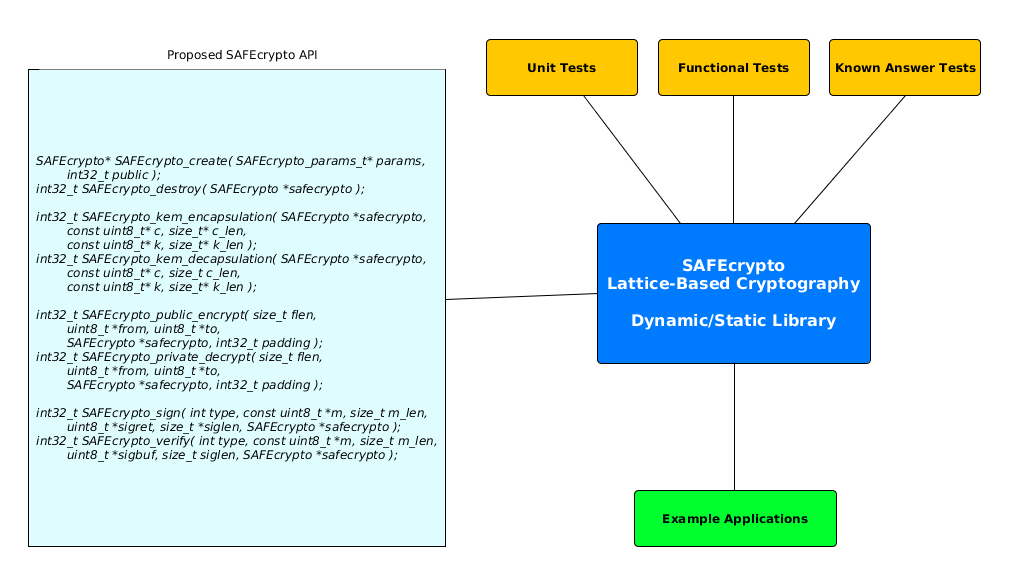
\includegraphics[scale=0.45]{../Resources/SAFEcrypto_structure.png}
\caption{Software structure}
\end{figure}


\section{Project Tools and Build Environment}

\subsection{Programming Language}

The SAFEcrypto software library will be written exclusively in C. In order to provide access to the compiled library in other programming languages a number of bindings will be provided. All C source code produced for the project will be C99 compliant, the ISO/IEC 9899:1999 version of the C programming language.


\subsection{Build Automation}

\textit{A presumption has been made that open-source tools will be preferred as they permit the build system to be deployed at a number of sites in the absence of a cost barrier.}

The build system will be capable of generating a package suitable for use on various platforms and microprocessor architectures with the primary focus being Linux. The generated package will be considered the output of Work Package 6 of the SAFEcrypto project.


\subsection{Code Repository}

The library will be developed at CSIT, as such it will utilise an Innersource GitLab repositiory hosted internally at CSIT as the revision control system for the SAFEcrypto project. In order to provide external access the library will be made publicly available using the SAFEcrypto GitHub repository, where both developers external to CSIT will be able to contribute to the project.


\subsection{Continuous Integration}

\href{https://jenkins.io/}{Jenkins} will be used as the project's CI tool. This will enable both rapid indentification of build errors and provide a consistent and maintainable system on which to create packages. Jenkins will be used to run all automated tests and build functionality, using email reports to notify users of errors.


\subsection{Build System}

The GNU Build System (Autotools) will be used to generate project packages. This build system will require the use of MinGW/MSYS in a Microsoft Windows environment.


\subsection{Compilers}

The GNU Compiler Collection (GCC) will be used on all platforms, using version 5.4 (released June 2016) as a minimum. This will be enforced as a rule within the automated build system to allow developers to standardise the compilation and linking of builds to a minimum standard.


\subsection{Dynamic Analysis Tools}

Dynamic program analysis is the analysis of computer software when running on a microprocessor, offering a user the facility to perform debug memory issues and profile the software. \href{http://valgrind.org/}{Valgrind} will be used to perform memory leak checking, using the test executables to provide sufficient code coverage for the dynamic analysis to be effective.


\subsection{Static Analysis Tools}

Static analysis is a technique that can improve the quality and reliability of software by analysing the source code. \href{http://www.splint.org/}{Splint} will be integrated into the build system for this purpose as an optional build target that developers can use to uncover potential problems.


\subsection{Software Style Formatters}

In order to help maintain a consistent coding style \href{https://www.gnu.org/software/indent/}{GNU Indent} will be used as part of the automated build system to improve the readability of the distributed source code by enforcing a coding style. The committed source code hosted by CSIT GitLab will not utilise automated software style formatting as this will lead to false positive version differences.


\subsection{Documentation Generators}

\href{http://www.doxygen.org/}{Doxygen} will be used for automated code documentation and generation of reference documentation.

\chapter{Coding Guidelines}
\label{ch_rules}

The software coding guidelines are segmented into three areas: the software version numbering system to be adopted, a \textit{style} guideline describing the general style that should be applied to all source code and \textit{coding rules} that must be adopted to promote software assurance.

\section{Version Numbering}

The following version numbering system will be employed:

\textbf{major.minor[.build[.revision]]}

\begin{itemize}
\item \textbf{major} --- Incremented when a major change occurs or the API is modified.
\item \textbf{minor} --- Incremented when a minor change in functionality occurs or a development milestone is reached. Reset to 0 when the major version number increments.
\item \textbf{build} --- Incremented every time the code is modified. Reset to 0 when the major or minor version number is increased.
\item \textbf{revision} --- Incremented when a previously released version is modified in some way to fix a bug or change its functionality.
\end{itemize}


\section{Style Guidelines}

\subsection{Enforced Rules}
A number of rules on coding style must be enforced in order to maintain the source code:

\begin{labeling}{100.}
\item [1.] \textbf{\textit{\#pragma once} should be used in favour of \textit{\#define} header guards.} \\
   Used to prevent multiple inclusion as \textit{\#define} header guards are prone to copy and paste errors. \\
\item [2.] \textbf{Include the defined legal statement with regards to software licensing in all source code files.} \\
   \begin{verbatim}
The MIT License (MIT)
Copyright (c) <year> <copyright holders>

Permission is hereby granted, free of charge, to any person obtaining a copy 
of this software and associated documentation files (the "Software"), to 
deal in the Software without restriction, including without limitation the 
rights to use, copy, modify, merge, publish, distribute, sublicense, and/or 
sell copies of the Software, and to permit persons to whom the Software is 
furnished to do so, subject to the following conditions:

The above copyright notice and this permission notice shall be included in 
all copies or substantial portions of the Software.

THE SOFTWARE IS PROVIDED "AS IS", WITHOUT WARRANTY OF ANY KIND, EXPRESS OR 
IMPLIED, INCLUDING BUT NOT LIMITED TO THE WARRANTIES OF MERCHANTABILITY, 
FITNESS FOR A PARTICULAR PURPOSE AND NONINFRINGEMENT. IN NO EVENT SHALL THE 
AUTHORS OR COPYRIGHT HOLDERS BE LIABLE FOR ANY CLAIM, DAMAGES OR OTHER 
LIABILITY, WHETHER IN AN ACTION OF CONTRACT, TORT OR OTHERWISE, ARISING 
FROM, OUT OF OR IN CONNECTION WITH THE SOFTWARE OR THE USE OR OTHER DEALINGS 
IN THE SOFTWARE.

\end{verbatim}
\item [3.] \textbf{The following copyright statement will be placed at the top of all source code files:}
\begin{verbatim}
/*****************************************************************************
 * Copyright (C) [INSTITUTION NAME], [YEAR]                                  *
 *                                                                           *
 * This file is part of libsafecrypto.                                       *
 *                                                                           *
 * This file is subject to the terms and conditions defined in the file      *
 * 'LICENSE', which is part of this source code package.                     *
 *****************************************************************************/
 \end{verbatim}
\item [4.] \textbf{Do not use git attributes or SVN keyword substitution.} \\
   This can lead to unnecessary file differences when working copies are updated, this in turn can lead to build systems performing unnecessary builds. \\
\item [5.] \textbf{To allow issues with source distributions to be tracked the distributed source code should contain tracking information that permits it to be related to the source code within the version control system. The following tagging information will be present in all source code files, when a source code distribution is built the tags will be modified by the build system with the relevant information.}
\begin{verbatim}
Git commit information:
  Author: $SC_AUTHOR$
  Date:   $SC_DATE$
  Branch: $SC_BRANCH$
  Id:     $SC_IDENT$
\end{verbatim}
\item [6.] \textbf{The limit on the length of lines is 80 columns.} \\
   Statements longer than 80 columns must be broken into sensible chunks, unless exceeding 80 columns significantly increases readability and does not hide information. Descendants are always substantially shorter than the parent and  are placed substantially to the right. The same applies to function headers with a long argument list. Never break user-visible strings, however, because that breaks the ability to grep for them. \\
\item [7.] \textbf{Use the defined SAFEcrypto data types} \\
   This will ease porting to different processor architectures. \\
\item [8.] \textbf{Always use the provided macros for dynamic memory allocation} \\
   These macros ensure that secure memory allocation is always undertaken, and can be easily modified when required to do so on a particular system. \\
\item [9.] \textbf{Use the provided debug macros} \\
   This is intended to allow development to place debug print statements in the
   source code that can be removed when a release library is built. \\
\item [10.] \textbf{Conditional statements should place a constant on the left} \\
   This is to prevent programming errors where assignments are implemented where the intention is to implement a test expression.
\end{labeling}


\subsection{Automated Rules}
Coding styles such as alignment, brackets and spacing can be manipulated by a CI script (using source code formatters) to ensure that source code committed to the revision system adheres to the style guidelines.

The following coding style is advised (adapted from the \href{https://www.openssl.org/policies/codingstyle.html}{OpenSSL Coding Style}) and will be enforced by automated tools when building a source distribution:

\begin{labeling}{100.}
\item [1.] \textbf{Use an adapted \textit{Kernighan and Ritchie} indent style.}
  
   \hspace{1cm} Functions are a special case where the opening bracket is at the start of the next line:
   \begin{verbatim}
        int function(int x)
        {
            body of function
        }
   \end{verbatim}
   \hspace{1cm} \textnormal{Condition statements:}
   \begin{verbatim}
        if (x_is_true) {
            do_y();
            do_z();
        }
   \end{verbatim}
   \hspace{1cm} \textnormal{Switch statements:}
   \begin{verbatim}
        switch (suffix) {
        case 'G':
        case 'g':
            mem <<= 30;
            break;
        case 'M':
        case 'm':
            mem <<= 20;
            break;
        case 'K':
        case 'k':
            mem <<= 10;
            /* fall through */
        default:
            break;
        }
   \end{verbatim}
   \hspace{1cm} Closing braces are not on an empty line of their own when followed by a continuation of the statement, but \textit{cuddled} braces will not be used:
   \begin{verbatim}
        do {
            ...
        } while (condition);

        if (x == y) {
            ...
        }
        else if (x > y) {
            ...
        }
        else {
            ...
        }
   \end{verbatim}
   \hspace{1cm} Always use braces around a single statement to help prevent copy and paste errors:
   \begin{verbatim}
        if (condition) {
            action();
        }
    
        if (condition) {
            do_this();
        }
        else {
            do_that();
        }
   \end{verbatim}
\item [2.] \textbf{Names with leading and trailing underscores should NOT be used.} \\
\item [3.] \textbf{\textit{\#define} constants and macros should be CAPITALISED.}
   \begin{verbatim}
        #define PARAM_THRESHOLD   5
   \end{verbatim}
\item [4.] \textbf{Enum constants should be CAPITALISED.}\\
   \begin{verbatim}
        typedef enum foobar {
            SC_ENUM_FOO = 0,
            SC_ENUM_BAR,
        } enum foobar\_e;
   \end{verbatim}
\item [5.] \textbf{Function, typedef, arguments and variable names, as well as struct, union and enum tag names should use underscore\_case.}\\
   \begin{verbatim}
        void function\_name(char *data_string, size_t len\_string);

        int variable\_name = 0;

        typedef struct my\_struct\_name my\_struct\_t;
   \end{verbatim}
\item [6.] \textbf{Global variables should use the prefix ``g\_''.}\\
\item [7.] \textbf{Pointer names should be positioned next to the ``*'' not the type name.}
   \begin{verbatim}
        int *pointer\_name;
   \end{verbatim}
\item [8.] \textbf{Use a space after C language keywords.}\\
\item [9.] \textbf{Do not add spaces around the inside of parenthesized expressions.}\\
\item [10.] \textbf{Use one space on either side of binary and ternary operators.}\\
\item [11.] \textbf{Do not put a space after unary operators.}\\
\item [12.] \textbf{Do not leave trailing whitespace at the ends of lines.}\\
\item [13.] \textbf{Separate functions with one blank line in the source file.}\\
\item [14.] \textbf{Always include parameter names with their data types in function prototypes.}\\
\item [15.] \textbf{In functions with complex return conditions and cleanup use the \textit{goto} statement as a mechanism to improve readability, reduce the possibility of errors and reduce excessive control structures.}
\item [16.] \textbf{To be continued\ldots}
\end{labeling}

\subsection{Doxygen Style}

Doxygen does not require any additional comments or special syntax added to source code in order to create reference documentation in the selected HTML, man pages or PDF.\@ However, developers can increase the usefulness of the reference documentation by adding comments and explanations directly to the source code using the required syntax.

Doxygen is very flexible in terms of the style that can be used to add documentation, however the following Doxygen style is encouraged for conformity. Developers can utilise more elaborate features of Doxygen if they desire to do so, e.g.\ describing function parameters and return values, grouping source files for documentation, etc.

\begin{labeling}{10.}
\item [1.] \textbf{Brief comment before}

Add an extra ``/''

\begin{verbatim}
    /// This method does something
    void DoSomething();
\end{verbatim}


\item [2.] \textbf{Brief comment after}

Add an extra ``/<''

\begin{verbatim}
    void DoSomething(); ///< This method does something
\end{verbatim}


\item [3.] \textbf{Detailed comment before}

Add an extra ``*'' [the intermediate leading ``*''s are optional]

\begin{verbatim}
    /** This is a method that does so much that I must
      * write an epic novel just to describe how much
      * it truly does. */
    void DoNothing();
\end{verbatim}


\item [4.] \textbf{Detailed comment after}

Add an extra ``*<'' [the intermediate leading ``*''s are optional]

\begin{verbatim}
    void DoNothing(); /**< This is a method that does so much
      * that I must write an epic novel just to describe how
      * much it truly does. */
\end{verbatim}

\end{labeling}


\newpage
\section{Coding Rules}

The following coding guidelines will be enforced using code reviews and automated rule checking with lint tools. The rules are segmented into three groups for clarity. Those rules that are not considered security specific, but are generic in nature and therefore applicable to the reliability and robustness of all software are given special consideration.

These rules have been derived from the SEI CERT C Coding Standard~\cite{sei_cert}. Developers are encouraged to familiarise themselves with this coding standard and use it as a reference when interpreting the rules given in this decoument. Other coding standards such as MISRA~\cite{misra_c} are also a useful resource.

\textbf{NOTE:} It is envisaged that to permit a pragmatic approach to development a \textit{debug} build of the package will be permitted for internal use that generates warnings rather than errors with regards to broken coding rules.

\subsection{Critical Security Rules}

\begin{labeling}{C.1000}
\item [C.1] Guarantee that library functions do not form invalid pointers [ARR38-C].
\item [C.2] Guarantee that storage for strings has sufficient space for character data and the null terminator [STR31-C].
\item [C.3] Do not pass a non-null-terminated character sequence to a library function that expects a string [STR32-C].
\item [C.4] Do not confuse narrow and wide character strings and functions [STR38-C].
\item [C.5] Exclude user input from format strings [FIO30-C].
\item [C.6] Distinguish between characters read from a file and \textit{EOF} or \textit{WEOF} [FIO34-C].
\item [C.7] Do not assume that \textit{fgets~()} or \textit{fgetws~()} returns a nonempty string when successful [FIO37-C].
\item [C.8] Do not call \textit{system~()} [ENV33-C].
\item [C.9] Call only asynchronous-safe functions within signal handlers [SIG30-C].
\item [C.10] Detect and handle standard library errors [ERR33-C].
\item [C.11] Properly seed pseudorandom number generators [MSC32-C].
\item [C.12] Do not pass invalid data to the \textit{asctime~()} function [MSC33-C].
\end{labeling}


\subsection{Important Security Rules}

\begin{labeling}{I.1000}
\item [I.1] Declare objects with appropriate storage durations [DCL30-C].
\item [I.2] Do not declare an identifier with conflicting linkage classifications [DCL36-C].
\item [I.3] Do not depend on the order of evaluation for side effects [EXP30-C].
\item [I.4] Do not access a volatile object through a nonvolatile reference [EXP32-C].
\item [I.5] Do not perform assignments in selection statements [EXP45-C].
\item [I.6] Ensure that unsigned integer operations do not wrap [INT30-C].
\item [I.7] Ensure that integer conversions do not result in lost or misinterpreted data [INT31-C].
\item [I.8] Ensure that operations on signed integers do not result in overflow [INT32-C].
\item [I.9] Ensure that division and remainder operations do not result in divide-by-zero errors [INT33-C].
\item [I.10] Do not use floating-point variables as loop counters [FLP30-C].
\item [I.11] Prevent or detect domain and range errors in math functions [FLP32-C].
\item [I.12] Do not attempt to modify string literals [STR30-C].
\item [I.13] Cast characters to unsigned char before converting to larger integer sizes [STR34-C].
\item [I.14] Use valid format strings [FIO47-C].
\item [I.15] Prevent data races when accessing bit-fields from multiple threads [CON32-C].
\item [I.16] Do not call \textit{signal~()} in a multithreaded program [CON37-C].
\item [I.17] Do not use the \textit{rand~()} function for generating pseudorandom numbers [MSC30-C].
\end{labeling}


\subsection{Minor Security Rules}

\begin{labeling}{M.1000}
\item [M.1] Avoid side effects in arguments to unsafe macros [PRE31-C].
\item [M.2] Do not use preprocessor directives in invocations of function-like macros [PRE32-C].
\item [M.3] Declare identifiers before using them [DCL31-C].
\item [M.4] Use the correct syntax when declaring a flexible array member [DCL38-C].
\item [M.5] Avoid information leakage when passing a structure across a trust boundary [DCL39-C].
\item [M.6] Do not modify objects with temporary lifetime [EXP35-C].
\item [M.7] Do not cast pointers into more strictly aligned pointer types [EXP36-C].
\item [M.8] Call functions with the correct number and type of arguments [EXP37-C].
\item [M.9] Do not modify constant objects [EXP40-C].
\item [M.10] Avoid undefined behavior when using restrict-qualified pointers [EXP43-C].
\item [M.11] Do not shift an expression by a negative number of bits or by greater than or equal to the number of bits that exist in the operand. [INT34-C]
\item [M.12] Use correct integer precisions [INT35-C].
\item [M.13] Always use \textit{intptr\_t} and \textit{uintptr\_t} to convert between integers and pointers [INT36-C].
\item [M.14] A pointer should store a pointer only, high order bits should not be used to store flags [INT36-C].
\item [M.15] Ensure that floating-point conversions are within range of the new type [FLP34-C].
\item [M.16] Preserve precision when converting integral values to floating-point type [FLP36-C].
\item [M.17] Do not use object representations to compare floating-point values [FLP37-C].
\item [M.18] Arguments to character-handling functions must be representable as an unsigned char [STR37-C].
\item [M.19] Allocate and copy structures containing a flexible array member dynamically [MEM32-C].
\item [M.20] Do not modify the alignment of objects by calling \textit{realloc~()} [MEM36-C].
\item [M.21] Do not return from a computational exception signal handler [SIG35-C].
\item [M.22] Do not rely on indeterminate values of errno [ERR32-C].
\end{labeling}


\subsection{Generic Rules}

\begin{labeling}{G.1000}
\item [G.1] All exit handlers must return normally [ENV32-C].
\item [G.2] Do not form or use out-of-bounds pointers or array subscripts [ARR30-C].
\item [G.3] Ensure size arguments for variable length arrays are in a valid range [ARR32-C].
\item [G.4] Free dynamically allocated memory when no longer needed [MEM31-C].
\item [G.5] Allocate sufficient memory for an object [MEM35-C].
\item [G.6] Do not alternately input and output from a stream without an intervening flush or positioning call [FIO39-C].
\item [G.7] Avoid TOCTOU (Time-of-Check to Time-of-Use) race conditions while accessing files [FIO45-C].
\item [G.8] Set errno to zero before calling a library function known to set errno, and check errno only after the function returns a value indicating failure [ERR30-C].
\item [G.9] Do not refer to an atomic variable twice in an expression [CON40-C].
\item [G.10] Ensure that control never reaches the end of a non-void function [MSC37-C].
\item [G.11] Do not declare or define a reserved identifier [DCL37-C].
\item [G.12] Reset strings on \textit{fgets~()} or \textit{fgetws~()} failure [FIO40-C].
\item [G.13] Do not call \textit{getc~(), putc~(), getwc~(),} or \textit{putwc~()} with a stream argument that has side effects [FIO41-C].
\item [G.14] Close files when they are no longer needed [FIO42-C].
\item [G.15] Only use values for \textit{fsetpos~()} that are returned from \textit{fgetpos~()} [FIO44-C].
\item [G.16] Do not modify the object referenced by the return value of certain functions [\textit{getenv~(), setlocale~(), locale-conv~(), asctime~(), or strerror~()}] [ENV30-C].
\item [G.17] Do not rely on an environment pointer following an operation that may invalidate it [ENV31-C].
\item [G.18] Do not store pointers returned by certain functions [\textit{getenv~(), asctime~(), localeconv~(), setlocale~(), and strerror~()}] [ENV34-C].
\item [G.19] Do not call \textit{signal~()} from within interruptible signal handlers.
\item [G.20] Clean up thread-specific storage [CON30-C].
\item [G.21] Use threadsafe C library functions in multithreaded code [CON33-C].
\item [G.22] Declare objects shared between threads with appropriate storage durations [CON34-C].
\item [G.23] Do not treat a predefined identifier as an object if it might only be implemented as a macro [\textit{assert, errno, math\_errhandling, setjmp, va\_arg, va\_copy, va\_end,} and \textit{va\_start}] [MSC38-C].
\end{labeling}


\bibliographystyle{unsrt}
\bibliography{coding}

\printindex

\end{document}
